\documentclass{article}
\usepackage{apacite}
\usepackage{hyperref}
\usepackage{multicol}
\usepackage{natbib}
\usepackage{sophia}
\usepackage[utf8]{inputenc}
\usepackage{array}
\setlength{\parindent}{0pt}
\usepackage{hyperref}

\usetikzlibrary{calc,patterns,angles,quotes}
\usepackage{pgfplots}
\pgfplotsset{width=15cm,height=10cm,compat=1.9}

\usepackage[english]{babel}
\usepackage{fancyhdr}
\usepackage{lastpage}
\pagestyle{fancy}
\fancyhf{}


\pagestyle{empty}% for cropping
\usepackage{tikz}
\usetikzlibrary{calc}
\usepackage{zref-savepos}
\usepackage{tabu}

\newcounter{NoTableEntry}
\renewcommand*{\theNoTableEntry}{NTE-\the\value{NoTableEntry}}

\newcommand*{\strike}[2]{%
  \multicolumn{1}{#1}{%
    \stepcounter{NoTableEntry}%
    \vadjust pre{\zsavepos{\theNoTableEntry t}}% top
    \vadjust{\zsavepos{\theNoTableEntry b}}% bottom
    \zsavepos{\theNoTableEntry l}% left
    \hspace{0pt plus 1filll}%
    #2% content
    \hspace{0pt plus 1filll}%
    \zsavepos{\theNoTableEntry r}% right
    \tikz[overlay]{%
      \draw
        let
          \n{llx}={\zposx{\theNoTableEntry l}sp-\zposx{\theNoTableEntry r}sp-\tabcolsep},
          \n{urx}={\tabcolsep},
          \n{lly}={\zposy{\theNoTableEntry b}sp-\zposy{\theNoTableEntry r}sp},
          \n{ury}={\zposy{\theNoTableEntry t}sp-\zposy{\theNoTableEntry r}sp}
        in
        (\n{llx}, \n{lly}) -- (\n{urx}, \n{ury})
      ;
    }% 
  }%
}

\usepackage{tikz}
\usetikzlibrary{calc}

\tikzset{
    right angle quadrant/.code={
        \pgfmathsetmacro\quadranta{{1,1,-1,-1}[#1-1]}     % Arrays for selecting quadrant
        \pgfmathsetmacro\quadrantb{{1,-1,-1,1}[#1-1]}},
    right angle quadrant=1, % Make sure it is set, even if not called explicitly
    right angle length/.code={\def\rightanglelength{#1}},   % Length of symbol
    right angle length=2ex, % Make sure it is set...
    right angle symbol/.style n args={3}{
        insert path={
            let \p0 = ($(#1)!(#3)!(#2)$) in     % Intersection
                let \p1 = ($(\p0)!\quadranta*\rightanglelength!(#3)$), % Point on base line
                \p2 = ($(\p0)!\quadrantb*\rightanglelength!(#2)$) in % Point on perpendicular line
                let \p3 = ($(\p1)+(\p2)-(\p0)$) in  % Corner point of symbol
            (\p1) -- (\p3) -- (\p2)
        }
    }
}
\pagestyle{fancy}
\fancyhf{}
\title{Projectile Motion Lab Report}
\author{Andi Xie}
\date{April 12, 2022}
\rfoot{Instructor: Mr. Sidhu}
\lhead{Student: Andi Xie}
\rhead{April 12, 2022}
\lfoot{SPH3U1 - 03}
\pagestyle{fancy}

 
\cfoot{Page \thepage \hspace{1pt} of \pageref{LastPage}}


\begin{document}

\maketitle
\tableofcontents
\newpage

\section{Overview}
\setcounter{page}{1}
The purpose of this experiment is to calculate the initial velocity (magnitude + direction) of the object when it is gently tossed from the hand from a video. The video only included the part that the object is in the air. Free-fall conditions will also be shown and proved during data analysis.

\section{Theory}
\label{theory}
The definition of acceleration is the change in velocity with respect to time. The formula is given from the slope of the Velocity-Time graph. Therefore this gives:
$$\Vec{a}=\frac{\Delta \Vec{v}}{\Delta t}$$
After rearranging the equation:
\begin{align*}
\Vec{a}&=\frac{\Delta \Vec{v}}{\Delta t}\\
  \Vec{a}&=\frac{\Vec{v_f}-\Vec{v_i}}{\Delta t}\\
  \Vec{a}\Delta t&=\Vec{v_f}-\Vec{v_i}\\
  \Vec{v_f}&=\Vec{v_i}+\Vec{a}\Delta t
\end{align*}

In words, the formula states that for every second during the movement, there is a change of $\Vec{a}$ added to $\Vec{v_i}$. After $\Delta t$ seconds, there is a total of $\Vec{a}\Delta t$ is added to $\Vec{v_i}$ to get $\Vec{v_f}$. Therefore $\Vec{v_f}=\Vec{v_i}+\Vec{a}\Delta t$.\\
This is similar to the slope of a $y=mx+b$ (linear) relationship:

\begin{align*}
    m&=\frac{\Delta y}{\Delta x}\\
    m&=\frac{y_2-y_1}{\Delta x}\\
    m\Delta x&=y_2-y_1\\
    y_2&=y_1+m\Delta x
\end{align*}
Therefore $\Vec{v_f}=\Vec{v_i}+\Vec a\Delta t$ is a $y=mx+b$ relationship.










\begin{center}
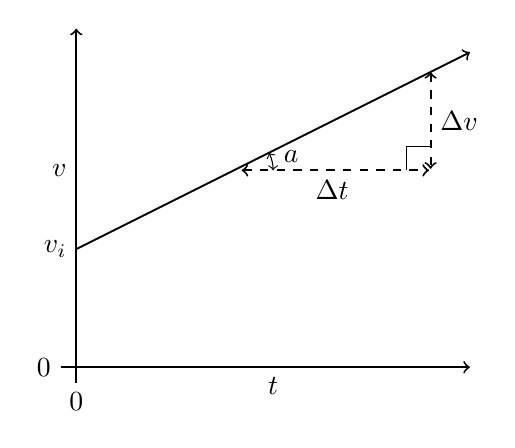
\begin{tikzpicture}[dot/.style={circle,inner sep=1pt,fill,label={#1},name=#1},
  extended line/.style={shorten >=-#1,shorten <=-#1},
  extended line/.default=1cm]
\draw[line width=.7pt,black,->] (-0.2,0)--(5,0);
\draw[line width=.7pt,black,->] (0,-0.2)--(0,4.3);
\draw[line width=.7pt,black,->] (0,1.5)--(5,4);
\draw[line width=.7pt,black,dashed,<->] (2.1,2.5)--(4.48,2.5);
\draw[line width=.7pt,dashed,black,<->] (4.5,3.75)--(4.5,2.52);


    \coordinate (vi) at (0,1.5);
    \coordinate (yLabel) at (0,3);
    \coordinate (xLabel) at (2.5,0);
    \coordinate (vf) at (4.5,3.75);
    \coordinate (vx) at (4.5,2.5);
    \coordinate (vy) at (2,2.5);
    
    \draw [right angle symbol={vx}{vy}{vf}];
    
\pic [draw, <->, "$a$", angle eccentricity=1.5] {angle = vx--vy--vf};


    \coordinate[label=left:$v$](c) at (0,2.5);
    \coordinate[label=left:$v_i$](c) at (vi);
    \coordinate[label=below:$t$](c) at (2.5,0);
    \coordinate[label=left:$0$](c) at (-0.2,0);
    \coordinate[label=below:$0$](c) at (0,-0.2);
    \coordinate[label=below:$\Delta t$](c) at (3.25,2.5);
    \coordinate[label=right:$\Delta v$](c) at (4.5,3.125);
    
    
\end{tikzpicture}
\end{center}










When an object is in motion, its acceleration can be splitted into the $x$ (horizontal) component and the $y$ (vertical) component. While the object is under free fall condition, gravity exerts a constant acceleration on the $y$ component towards the ground. But this has no effect to the $x$ component if we neglect air resistance. According the article of \cite{clay2004pendulum} from the American Association of Physics Teachers, the gravity downward acceleration is $9.8$ m/s$^2$ towards the ground.



\section{Variables}
The lab involves time, velocity, acceleration.
\begin{center}
    \begin{tabular}{|c||c|c|c|c|c|c|c|}\hline 
            \strike{|c||}{} & $t$         & $\Vec{v_x}$     & $\Vec{v_y}$      & $\Vec{v_i}$       & $\Vec{v_f}$     & $\Vec{a}$        \\\hline 
        Type & Independent & Dependent & Dependent  & Controlled  & Dependent & Controlled \\\hline 
        Unit & s         & m/s     & m/s      & m/s       & m/s     & m/s$^2$    \\\hline
    \end{tabular}
\end{center}


\section{Data Processing}
The velocity of each frame is calculated by the built-in feature of tracker. The data is later plotted into a Velocity-Time graph of the object. I will be using linear equation to graph. The slope of the graph would be the acceleration.



$\Vec{v_f}=\Vec{a}\Delta t+\Vec{v_i}$ is a graph of $y=mx+b$, $t$ is the independent variable, both $\Vec{a}$ and $\Vec{v_i}$ is given, and $\Vec{v_f}$ is the dependent variable.\\
\begin{itemize}
    \item $y$ is $\Vec{v_f}$, with unit of m/s
    \item $m$ is $\Vec a$, with unit of m/s$^2$
    \item $x$ is $t$, with unit of s
    \item $b$ is $\Vec{v_i}$, with unit of m/s
\end{itemize}

The unit of the slope would be:
\begin{align*}
    &\frac{\frac{\text{m}}{\text{s}}-\frac{\text{m}}{\text{s}}}{\text{s}}\\
    =\ &\frac{\frac{\text{m}}{\text{s}}}{\text{s}}\\
    =\ &\frac{\text{m}}{\text{s}^2}
\end{align*}
Which matches the unit in the \hyperref[theory]{theory} section. 



\pagebreak
\section{Apparatus}
Materials used in the experiment:
\begin{itemize}
    \item pen cap
    \item phone for video taping
    \item table
\end{itemize}

\section{Procedure}
\begin{enumerate}
    \item Put the camera (phone) to an appropriate height and angle
    \item Record the process of throwing the cap
    \item Edit the video, only leave the free fall section
    \item Import the video to tracker
    \item Track the points, calibrate
    \item Export the velocity data to \LaTeX
    \item Make Velocity-Time graphs with \LaTeX 
\end{enumerate}
Upward and the right side will be the positive direction throughout this experiment

\pagebreak
\section{Observations}
\subsection{Raw Data}
Data from tracker:
\renewcommand{\arraystretch}{2}
\begin{center}
    \begin{tabular}{|m{1.4cm}|m{1.4cm}|m{1.4cm}|}
    \hline
$t\ (\text s)$&	$\Vec{v_x}$ (m/s)&	    $\Vec{v_y}$ (m/s)\\\hline 
0&   \strike{c}{}&    	\strike{|c|}{}\\\hline 
0.0334& 1.55&	1.67\\\hline 
0.0667& 1.48&	1.36\\\hline 
0.1&    1.51&	1.00\\\hline 
0.133&	1.54&	0.622\\\hline 
0.167&	1.51&	0.255\\\hline 
0.2&	1.52&	-0.113\\\hline 
0.234&	1.49&	-0.461\\\hline 
0.267&	1.39&	-0.774\\\hline 
0.3&	1.38&	-1.06\\\hline 
0.334&	1.41&	-1.31\\\hline 
0.367&	1.40&	-1.61\\\hline 
0.4&	1.44&	-1.97\\\hline 
0.434&	1.48&	-2.22\\\hline 
0.467&	1.46&	-2.63\\\hline 
0.5&	1.52&	-3.05\\\hline 
0.534&	1.62&	-3.36\\\hline 
0.567&	1.57&	-3.67\\\hline 
0.601&	1.50&	-3.84\\\hline 
0.634&	\strike{c}{}	&   \strike{|c|}{}\\ \hline 
    \end{tabular}
    \end{center}
    



\pagebreak
Make a chart with these data:
\begin{center}
\begin{tikzpicture}
\begin{axis}[
    enlargelimits=false,
    title={Velocity vs. Time},
    xlabel={Time (s)},
    ylabel={Velocity (m/s)},
    xmin=0, xmax=0.6,
    ymin=-4, ymax=2,
    xtick={0,0.1,0.2,0.3,0.4,0.5,0.6},
    ytick={-4,-3,-2,-1,0,1,2},
    legend pos=south west,
    ymajorgrids=true,
    xmajorgrids=true,
    grid style=dashed,
]
\addplot[
    color=blue,
    only marks,
    mark=square,]
table[meta=Vx]
{Data.dat};

\addplot[
    color=red,
    only marks,
    mark=square,]
table[meta=Vy]
{yData.dat};


\addplot [
    domain=0:0.6, 
    samples=100, 
    color=black,
    ]
{0.0000000000000000001*x};


\addplot [
    domain=0:0.6, 
    samples=100, 
    color=blue,
    ]
{0.0152*x+1.48};
\addlegendentry{\(\Vec{v_x}=0.0152t+1.48\)}

\addplot [
    domain=0:0.6, 
    samples=100, 
    color=red,
    ]
    {-9.81*x+1.93};
\addlegendentry{\(\Vec{v_y}=-9.81t+1.93\)}


\end{axis}
\end{tikzpicture}
\end{center}





\subsection{Data Analysis}
Label the equations for reference:
\begin{equation} 
    \Vec{v_x}\text{ [m/s] }=0.0152\text{ [m/s}^2\text{] }\cdot t\text{ [s] }+1.48\text{ [m/s] }\label{vx}
\end{equation}
\begin{equation} 
    \Vec{v_y}\text{ [m/s] }=-9.81\text{ [m/s}^2\text{] }\cdot t\text{ [s] }+1.93\text{ [m/s] }\label{vy}
\end{equation}

In the $x$ (horizontal) direction, equation \ref{vx} has a slope close to $0$, error is negligible. Slope of 0 indicates that the horizontal velocity did not change over time, which means the acceleration $\Vec a=0$.\\\\
In the $y$ (vertical) direction, equation \ref{vy} has a slope of $9.81$. The $y$-intercept always has $x=0$, which means this is at initial condition, indicates $\Vec{v_i}$.\\

\newpage

The percentage difference is given by the formula:
\[
\text{Percentage Difference }=\left|\frac{\text{Experimental Result }-\text{ Theoretical Result}}{\text{Theoretical Result}}\right|\times 100\%
\]

Calculate the percentage error of the experimental gravitational acceleration constant from $9.81$ m/s$^2$:

\begin{align*}
    &\left|\frac{9.81-9.81}{9.81}\right|\times 100\%\\
    =\ &\frac{0}{9.81}\times 100\%\\
    =\ &0\%
\end{align*}
The object was falling at the same acceleration as the data provided by \cite{clay2004pendulum}, free fall condition is proven.



\subsection{Compute the Initial Velocity}
Based on the data from the graph, $\Vec{v_{ix}}=1.48$ m/s and $\Vec{v_{iy}}=1.93$ m/s. Construct a right triangle with these side lengths:

\begin{center}
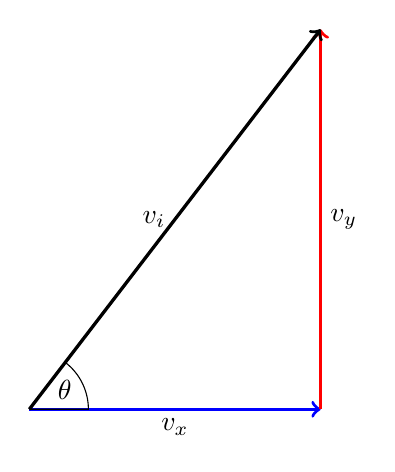
\begin{tikzpicture}
\draw[line width=1.2pt,blue,->] (0,0)--(3.7,0);
\draw[line width=1.2pt,red,->] (3.7,0)--(3.7,4.825);
\draw[line width=1.2pt,black,->] (0,0)--(3.7,4.825);


    \coordinate (A) at (0,0);
    \coordinate (B) at (3.7,0);
    \coordinate (C) at (3.7,4.825);

    \coordinate[label=below:$\Vec{v_x}$](c) at ($ (A)!.5!(B) $);
    \coordinate[label=left:$\Vec{v_i}$] (b) at ($ (A)!.5!(C) $);
    \coordinate[label=right:$\Vec{v_y}$](a) at ($ (B)!.5!(C) $);
    
     \draw (0,0) -- (0:0.75cm) arc (0:52:.75cm);
    \draw (0.45cm,0.25cm) node {$\theta$};
\end{tikzpicture}
\end{center}


Calculate the magnitude, from Pythagoras Theorem:
\begin{align*}
    \left(\Vec{v_i}\right)^2&=\left(\Vec{v_x}\right)^2+\left(\Vec{v_y}\right)^2\\
    \Vec{v_i}&=\sqrt{1.48^2+1.93^2}\\
    \Vec{v_i}&\approx 2.43\text{ m/s}
\end{align*}

Let $\theta$ be the angle between $\Vec{v_i}$ and $\Vec{v_x}$, from trigonometric function:
\begin{align*}
    \tan \theta&=\frac{\Vec{v_y}}{\Vec{v_x}}\\
    \theta&=\tan^{-1}\left(\frac{1.93}{1.48}\right)\\
    \theta&\approx 53^\circ
\end{align*}

\pagebreak
\section{Conclusion \& Evaluation}
From the experiment, the pen cap was tossed $53^\circ$ above the horizontal with a velocity of $2.43$ m/s initially (or $2.43$ m/s $\left[\text{E } 53^\circ \text{ N}\right]$). During the time in the air, if neglect air resistance, the cap is accelerating $9.81$ m/s$^2$ towards the ground. Free fall condition is proven.

\section{Factors Affecting the Accuracy Of the Experiment}

Angle of the camera is the biggest factor that affects the accuracy in the experiment. The camera delivers the most accurate video only when it is pointed perpendicular to the plane and the object is at the point of intersection. Which means the camera would have to move along with the object. For a counter example, if the camera is pointed in the same direction as the object is moving, the result will show $v_x=0$\\\\
There are other factors such as accuracy of tracking the points, stability of the camera, ruler I was holding being further to the camera than the object, and air resistance. But Angle of the camera is by far the most prominent.


\bibliographystyle{apacite}
\bibliography{References}
\end{document}
